\documentclass{article} %standard document class available with Latex
\usepackage{fancyhdr} %Package for including headers and footers
\usepackage{graphicx}

%Details for the title page
\title{My First Report}
\author{Primal}
\date{February 20 2012}

\pagestyle{fancy} %To remove header on title document
\lhead{\footnotesize Left Header} %left header
\lfoot{\footnotesize Left Footer } %left footer
\cfoot{\footnotesize Central Footer} %Central footer
\rhead{\footnotesize Right Header} %Right Header
\rfoot{\footnotesize Right Footer} %Right Footer

\begin{document}
\maketitle %Generates the title page. Should be after \begin{document}
\abstract{This is a summary of the report. At the moment there's not much to say} %Generates abstract as you would imagine 
\tableofcontents %Generates the table of contents out of the box
\section{Introduction}
Hello!  Here's some text.

To make a new paragraph, just leave a blank line.

\subsection{Background theory}
More about this later

\section{Apparatus}
Test-tubes and so on.

\section{formatting}
This is an example of \textit{italicized} text. To have 
tiny {\tiny text} to huge {\huge text} use the tiny, small, large,
huge in that order.

\section{Listing}

\begin{itemize}
\item Unnumbered
\item List 
\item Items
\end{itemize}

\begin{enumerate}
\item Numbered
\item List 
\item Items
\end{enumerate}


\section{Figures}
\begin{figure}[htbp]
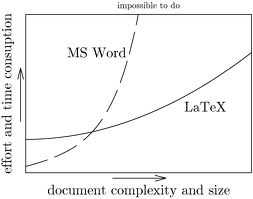
\includegraphics[width=10cm]{latex.jpeg}
\caption{Latex Rocks}
\label{LATEX}
\end{figure}

\end{document}
